\chapter{Real Zeros}\label{ch:zeros}\index{Lee Yang property}\index{Malo's theorem}\index{real zeros}\index{P\'olya frequency sequence}

Chapter~\ref{ch:counts} left a question: on what class of laws does the exact ladder act well? Its Section~\ref{ch:kingman} showed that log concavity of the count is not the answer to the question of monotonicity. This chapter proposes an answer to the question of invariance, a Lee Yang property \cite{LY52} for the ladder. The heat kernel is a product $\prod_m(1+x/\gamma_m)$ with every $\gamma_m\ge1$: as a function of $x=\cos\theta$ all of its zeros are real and lie to the left of $-1$. We prove that heat flow on the group preserves this property, that the coalescence of Theorem~\ref{thm:coalescence} has it, and we give evidence that the whole exact ladder does.

\section{Two classes}\label{sec:twoclasses}

\begin{definition}
Let $\mathcal L$ be the set of class functions on SU(2) of the form $\rho(x)=c\prod_m(1+x/\gamma_m)$ with $c>0$, $\gamma_m\ge1$ and $\sum_m1/\gamma_m<\infty$, together with their locally uniform limits. Let $\mathcal L'$ be the set of derivatives $F'$, in the variable $x$, of functions $F\in\mathcal L$.
\end{definition}

A member of $\mathcal L$ is an entire function of $x$ whose zeros are all real and at most $-1$; in the variable $z=e^{i\theta}$ its zeros are negative real numbers, in pairs $-e^{\pm\eta}$ with $\gamma=\cosh\eta$. Since $1+x/\gamma=(1-\frac1\gamma)+\frac1\gamma(1+x)$, every member of $\mathcal L$ lies in the family $\mathcal M$ of Chapter~\ref{ch:counts}, with a count $M_0$ that is a sum of independent Bernoulli variables of parameters $1/\gamma_m$; by the theorem of Aissen, Schoenberg, Whitney and Edrei~\cite{Ed52} these are exactly the members of $\mathcal M$ whose count $\nu_0$ is a P\'olya frequency sequence with an entire generating function \cite{ASWE}. By Rolle's theorem $\mathcal L'\subset\mathcal L$.

Three examples. The densities $f_a\propto(1+x)^a$ are in $\mathcal L'$, with $F=(1+x)^{a+1}$. The heat kernel is in $\mathcal L'$: the proof of Theorem~\ref{thm:product} gave $K_t=\frac12\partial_x\vartheta$ with $\vartheta\propto\prod_n(C_n+x)$, so the antiderivative of the heat kernel in $\cos\theta$ is the theta function, which is in $\mathcal L$. The Wilson law $e^{\kappa x}=\lim(1+x/\gamma)^{\kappa\gamma}$ is in the closure of both.

\section{Convolution on SU(2) through the circle}\label{sec:circlecv}

\begin{lemma}\label{lem:circle}
Let $f=\sum_na_n\chi_n$ and $g=\sum_nb_n\chi_n$ be class functions and let $G$ be any antiderivative of $g$ in $x$. Write $\tilde f(z)=f\cdot(z-z^{-1})=\sum_{n\ne0}\operatorname{sgn}(n)\,a_{|n|}z^n$ and $G=\sum_n\hat G_nz^n$. Then $\hat G_n=b_{|n|}/(2|n|)$ for $n\ne0$, and
\[
\widetilde{f*g}(z)=2\sum_{n\ne0}\tilde f_n\,\hat G_n\,z^n .
\]
If also $f=F'$, then $f*g$ is a constant multiple of the derivative in $x$ of the convolution of $F$ and $G$ on the circle.
\end{lemma}

\begin{proof}
$\chi_n=T_n'/n$ with $T_n(\cos\theta)=\cos n\theta$, so $G=\sum_n(b_n/n)\,T_n$ up to a constant, which gives $\hat G_n$. Convolution on the group sends $(a_n,b_n)$ to $a_nb_n/n$, and $\operatorname{sgn}(n)a_{|n|}b_{|n|}/|n|=2\tilde f_n\hat G_n$. The constant term of $G$ plays no part because $\tilde f_0=0$.
\end{proof}

So the convolution of class functions on SU(2) is a Hadamard product of Laurent coefficients, of one function multiplied by $z-z^{-1}$ and an antiderivative of the other. For Hadamard products there is a classical theorem.

\begin{theorem}[Malo \cite{Malo}]\label{thm:malo}
If $P(z)=\sum_ka_kz^k$ has only real zeros and $Q(z)=\sum_kb_kz^k$ has only real zeros, all of the same sign, then $\sum_ka_kb_kz^k$ has only real zeros.
\end{theorem}

\section{What is proved}

\begin{theorem}[real zeros under convolution]\label{thm:zeros}
\begin{enumerate}
\item[(i)] If $f\in\mathcal L$ and $g\in\mathcal L'$ are polynomials with $\deg f\le\deg g$, then $f*g\in\mathcal L$.
\item[(ii)] If $f,g\in\mathcal L'$ are polynomials, then $f*g\in\mathcal L'$.
\item[(iii)] If $f\in\mathcal L$ and $t>0$, then $f*K_t\in\mathcal L$: heat flow on SU(2) preserves the class.
\end{enumerate}
\end{theorem}

\begin{proof}
(i) Let $G\in\mathcal L$ be an antiderivative of $g$, of degree $D=\deg g+1$ in $x$. Then $Q(z)=z^DG$ is a polynomial with only negative zeros, and $P(z)=z^D\tilde f$ is a polynomial, because $\deg f+1\le D$, whose zeros are those of $f$, which are negative, together with $\pm1$ and possibly $0$: all real. By Lemma~\ref{lem:circle} the Hadamard product of $P$ and $Q$ is $\frac12z^D\,\widetilde{f*g}$, which by Malo's theorem has only real zeros. So $f*g$ has only real zeros in $z$, that is, zeros in $x$ that are real and outside $(-1,1)$. Since $f*g$ lies in $\mathcal M$ it is positive for $x>-1$; the zeros are therefore at most $-1$.

(ii) Order the two so that $\deg F\le\deg G$. The Hadamard product of $z^DF$ and $z^DG$ has only real zeros by Malo's theorem and positive coefficients, so the convolution of $F$ and $G$ on the circle is in $\mathcal L$, and by the lemma $f*g$ is its derivative up to a constant.

(iii) For a polynomial $f$, approximate $\vartheta$ by its partial products, which are in $\mathcal L$ and of degree as high as we please, apply (i), and pass to the limit by Hurwitz's theorem. A general $f\in\mathcal L$ is a locally uniform limit of polynomials $f_N\in\mathcal L$ (finite products, or their limits), and we show that $f_N*K_t\to f*K_t$ locally uniformly in complex $x$. Write $x=(z+z^{-1})/2$, let $R>1$, and let $E_R$ be the ellipse that is the image of $|z|=R$. If $F$ is entire in $x$, the Laurent coefficients $\hat F_n$ of $F\big((z+z^{-1})/2\big)$ satisfy $|\hat F_n|\le\max_{E_R}|F|\,R^{-|n|}$ by Cauchy's estimate. Comparing the coefficients of $z^n$ in $F(x)(z-z^{-1})=\sum_{n\ge1}a_n(z^n-z^{-n})$ gives $a_n=\hat F_{n-1}-\hat F_{n+1}$ for the character coefficients $F=\sum a_n\chi_n$, so $|a_n|\le2R\max_{E_R}|F|\,R^{-n}$, and therefore $\sup_nR^n|a_n(f_N)-a_n(f)|\le2R\max_{E_R}|f_N-f|\to0$. The coefficients of $f*K_t$ are $a_ne^{-(n^2-1)t/4}$, and $|\chi_n|\le nR^{n-1}$ on $E_R$, so
\[
\max_{E_R}|f_N*K_t-f*K_t|\le\sup_nR^n|a_n(f_N)-a_n(f)|\sum_{n\ge1}n\,e^{-(n^2-1)t/4}\to0 .
\]
Every compact set lies in some $E_R$, so $f*K_t$ is a locally uniform limit of the functions $f_N*K_t$, which are in $\mathcal L$ by the polynomial case. By the definition of $\mathcal L$, which contains its locally uniform limits, $f*K_t\in\mathcal L$.
\end{proof}

\begin{corollary}[the coalescence has real zeros]\label{cor:coalzeros}
For all integers $a,b\ge0$,
\[
f_a*f_b=c\prod_{i=1}^{\min(a,b)}\Big(1+\frac{x}{\gamma_i(a,b)}\Big),\qquad\gamma_i(a,b)\ge1 .
\]
Hence the count $M_0$ of $f_a*f_b$ is a sum of $\min(a,b)$ independent Bernoulli variables, and the sequence $j\mapsto Q(j\mid a,b)\,2^j/C_{j+1}$ is a P\'olya frequency sequence: in particular it is log concave and unimodal.
\end{corollary}

For example $f_3*f_3$ has zeros $-1.394$, $-3.443$ and $-19.16$. The corollary strengthens Theorem~\ref{thm:coalescence}: the weights of the coalescence kernel are not only positive, after division by $C_{j+1}2^{-j}$ they are the coefficients of a polynomial with only real zeros.

Part (iii) is a statement of the kind that de Bruijn proved on the line \cite{dB50} and that runs through our Riemann volumes: the forward heat flow preserves the reality of zeros. Here the flow is Brownian motion on the group, the variable is $\cos\theta$, and the zeros stay real and to the left of $-1$. In the language of Section~\ref{ch:langlands}, every factor stays Ramanujan under heat flow. In the language of Section~\ref{ch:kingman}, the death process of Kingman's coalescent maps sums of independent Bernoulli counts to sums of independent Bernoulli counts.

\section{An exact case: two Wilson laws}\index{Gegenbauer addition theorem}

One convolution can be done in closed form, and it shows the theorem at work on laws that are not polynomials.

\begin{proposition}[Wilson times Wilson]\label{prop:wilsonwilson}
For $\kappa,\lambda>0$,
\[
e^{\kappa x}*e^{\lambda x}=\frac{2I_1(r)}{r},\qquad r^2=\kappa^2+\lambda^2+2\kappa\lambda x .
\]
Its zeros in $x$ are
\[
x_m=-\frac{\kappa^2+\lambda^2+j_{1,m}^2}{2\kappa\lambda}\ \le\ -1-\frac{j_{1,m}^2}{2\kappa\lambda},\qquad m=1,2,\dots,
\]
where $j_{1,m}$ are the positive zeros of the Bessel function $J_1$. So the convolution of two Wilson laws is in $\mathcal L$, with $\gamma_m=(\kappa^2+\lambda^2+j_{1,m}^2)/(2\kappa\lambda)$, and its count is a sum of independent Bernoulli variables with parameters $2\kappa\lambda/(\kappa^2+\lambda^2+j_{1,m}^2)$.
\end{proposition}

\begin{proof}
Identify SU(2) with the unit sphere of the quaternions, so that $\frac12\operatorname{tr}(V^{-1}U)=\langle V,U\rangle$. Then $(e^{\kappa x}*e^{\lambda x})(U)=\int\exp\langle V,\kappa+\lambda U\rangle\,dV$, the integral of a plane wave over $S^3$, which is $2I_1(|A|)/|A|$ with $A=\kappa+\lambda U$ and $|A|^2=\kappa^2+\lambda^2+2\kappa\lambda\,a_0(U)$. The function $I_1(r)/r$ is even and entire in $r$ with zeros at $r=\pm ij_{1,m}$.
\end{proof}

This is Gegenbauer's addition theorem for Bessel functions in the form it takes on the group. In characters, $e^{\kappa x}=\sum_n(2n/\kappa)I_n(\kappa)\chi_n$, so the statement is $2I_1(r)/r=\sum_n(4n/\kappa\lambda)\,I_n(\kappa)I_n(\lambda)\,\chi_n(x)$, which we also checked numerically to forty figures (\texttt{zeros\_checks.py}). Three things follow.

The zeros are real and to the left of $-1$ by inspection, as Conjecture~\ref{conj:Lclosed} predicts, and the edge $-1$ is attained only in the limit $\kappa\lambda\to\infty$.

The first half of the first rung from a Wilson law is explicit. Bond moving sends $\kappa$ to $k\kappa$ exactly, and one convolution then gives the law $2I_1(r)/r$ with $r=2k\kappa\cos(\theta/2)$: a function of $y=\cos^2(\theta/2)$ alone, with largest zero at $-\gamma_1$, $\gamma_1=1+j_{1,1}^2/(2k^2\kappa^2)$ and $j_{1,1}=3.8317$. For $k\kappa=4$ this is $\gamma_1=1.459$. The zeros have come in from infinity, as Section~\ref{ch:kingman} observed in the count, and the Bernoulli parameters $1/\gamma_m$ of the count are explicit.

The count of this law has a name as well. Expanding, $2I_1(r)/r=\sum_m(r/2)^{2m}/(m!\,(m+1)!)$ with $(r/2)^2=\frac12k^2\kappa^2(1+x)$, so $\nu_0(m)\propto(k^2\kappa^2/2)^m/(m!\,(m+1)!)$: where the Wilson law has a Poisson count, its convolution square has a count with weights $c^m/(m!\,(m+1)!)$, the law of the smaller coordinate of a pair of independent Poisson variables conditioned to differ by one. The product formula for $I_1$ then says that this law is a sum of independent Bernoulli variables, a fact about Bessel numbers that we have not seen stated in this way.

\section{The Thorin form: are Wilson laws generalized gamma convolutions?}\index{generalized gamma convolution}\index{Thorin measure}\index{Hartman Watson law}

The class $\mathcal L$ is the class of this book's title in another variable. If $\rho=c\prod_m(1+x/\gamma_m)$ then
\[
\frac{\rho(0)}{\rho(x)}=\prod_m\frac{\gamma_m}{\gamma_m+x}=\E\,e^{-xT_\rho},\qquad T_\rho=\sum_m\frac{E_m}{\gamma_m},
\]
with independent standard exponential $E_m$. So the reciprocal of a member of $\mathcal L$, as a function of $x=\cos\theta$, is the Laplace transform of a generalized gamma convolution whose Thorin measure \cite{Th77,Bo92} $U_\rho=\sum_m\delta_{\gamma_m}$ has integer masses and is supported on $[1,\infty)$, beyond the edge of the group; limits add a drift. In this dictionary:
\begin{center}
\small
\begin{tabular}{p{0.34\textwidth}p{0.58\textwidth}}
\toprule
law of a link & Thorin measure of $T_\rho$ \\ \midrule
Haar measure & zero \\
$f_a\propto(1+x)^a$ & $a\,\delta_1$, a gamma law of shape $a$ \\
heat kernel $K_t$ & $\sum_m\delta_{\gamma_m(t)}$, atoms moving to the right as $t$ grows \\
Wilson law $e^{\kappa x}$ & zero, with drift $\kappa$: the point mass at $\kappa$ \\
Wilson convolved with Wilson & $\sum_m\delta_{\gamma_m}$, $\gamma_m=(\kappa^2+\lambda^2+j_{1,m}^2)/(2\kappa\lambda)$ \\
bond moving, power $k$ & $U\mapsto kU$, the sum of $k$ independent copies of $T$ \\
heat flow & a map of integer Thorin measures on $[1,\infty)$ to themselves (Theorem~\ref{thm:zeros}) \\
\bottomrule
\end{tabular}
\end{center}
The offset of the Thorin measure, the quantity the first chapters of this book were written about, is $\gamma_1$, the negative of the largest zero, and Conjecture~\ref{conj:Lclosed} below says that convolution on the group acts on integer Thorin measures supported on $[1,\infty)$.

So are Wilson laws related to generalized gamma convolutions? In four ways, of which the first is degenerate and the last is a negative.

\emph{As the boundary case.} The reciprocal of the Wilson law is $e^{-\kappa x}$, the Laplace transform of a point mass: a generalized gamma convolution with no Thorin measure, only drift. The Wilson family is the edge of $\mathcal L$ at which all the atoms have gone to infinity. This is why bond moving costs it nothing and why it has no curvature loss.

\emph{After one convolution.} By Proposition~\ref{prop:wilsonwilson} the reciprocal of $e^{\kappa x}*e^{\lambda x}$ is $r/(2I_1(r))$ with $r^2=\kappa^2+\lambda^2+2\kappa\lambda x$. Chapter~\ref{ch:kacyang} identifies $\sqrt{2s}/(2I_1(\sqrt{2s}))$ as the Laplace transform of the hitting time $\tau$ of the unit sphere $S^3$ by Brownian motion in $\mathbb R^4$, a generalized gamma convolution with Thorin atoms at $\frac12j_{1,m}^2$. Hence
\[
\frac{1}{(e^{\kappa x}*e^{\lambda x})(x)}=\E\Big[e^{-(\kappa^2+\lambda^2)\tau/2}\,e^{-\kappa\lambda\tau\,x}\Big],
\]
the Laplace transform in $x$ of $\kappa\lambda\tau$ under an exponential tilt, and tilting a generalized gamma convolution shifts its Thorin atoms and keeps it in the class. The one plaquette partition function of that chapter is the case $x=1$, $\kappa=\lambda$.

\emph{As a mixture of heat kernels.} The character coefficients of the Wilson law are $u_n=I_n(\kappa)/I_1(\kappa)$. Hartman and Watson \cite{HW74} showed that $I_{\sqrt{2s}}(\kappa)/I_0(\kappa)$ is the Laplace transform of a probability law $\Xi_\kappa$ on the half line, which now carries their names and which Yor \cite{Yor80} found in the windings of planar Brownian motion. Therefore
\[
\frac{I_n(\kappa)}{I_1(\kappa)}=\int e^{-(n^2-1)\xi/2}\,\tilde\Xi_\kappa(d\xi),\qquad\frac{e^{\kappa x}}{Z(\kappa)}=\int K_{2\xi}\,\tilde\Xi_\kappa(d\xi),
\]
with $\tilde\Xi_\kappa$ the Hartman Watson law tilted by $e^{-\xi/2}$: the Wilson law is a mixture of heat kernels over a random time. The Hartman Watson law is infinitely divisible, and it is known to lie in the Bondesson class \cite{Ke78,Bo92}, whose members have a complete Bernstein function as the negative logarithm of the Laplace transform; that class contains the generalized gamma convolutions. This mixture is the original theorem of Hartman and Watson, whose title speaks of normal distribution functions on spheres: the von Mises Fisher law on a sphere, which on $S^3$ is the Wilson law, is a mixture of the Brownian, or normal, laws on the sphere, which are the heat kernels. Hartman's paper of 1976 \cite{Har76} on completely monotone families of solutions of linear differential equations then gave the general mechanism, for Bessel functions and beyond, by which such ratios are Laplace transforms of infinitely divisible laws; read in the language of our Riemann volumes it is a scale mixture of normals result of the extended generalized gamma convolution kind, with the heat kernel in the part of the normal law and the Hartman Watson time in the part of the mixing variance. Whether the Hartman Watson law is itself a generalized gamma convolution in the strict sense is settled in the next section. It is one, with an explicit Thorin measure, and the Wilson action is a Thorin mixture of heat kernel actions.

\emph{As a law on the group, no.} The law of $1-\cos\theta$ under the Wilson measure lives on $[0,2]$, and a nondegenerate generalized gamma convolution has unbounded support. Only in the weak coupling scaling does it become one: $\kappa(1-\cos\theta)$ tends to a gamma law of shape $\frac32$.

\begin{figure}[t]
\centering
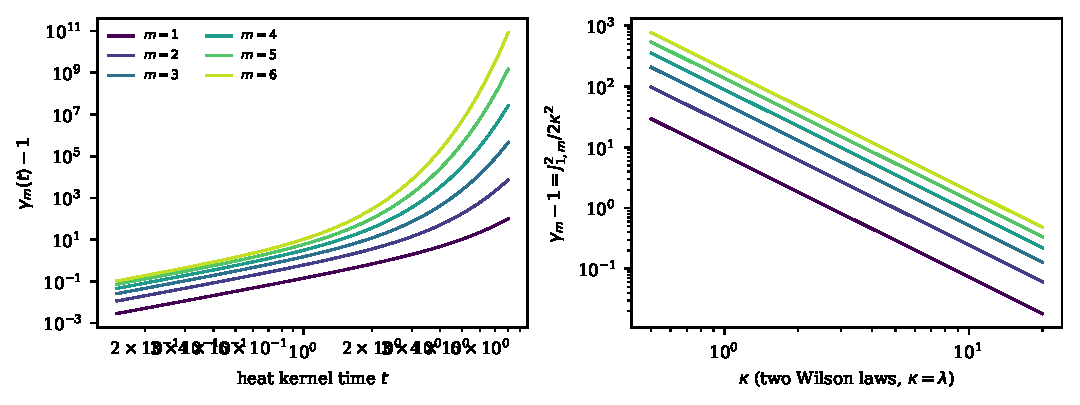
\includegraphics[width=\textwidth]{figures/zeros_fig.pdf}
\caption[Zeros of the heat kernel and of two Wilson laws]{The Thorin atoms $\gamma_m$, shown as $\gamma_m-1$, the distance of the zeros of the link density from the edge $\cos\theta=-1$. Left: the first six for the heat kernel, increasing in $t$. Right: for the convolution of two Wilson laws of equal coupling, where $\gamma_m-1=j_{1,m}^2/2\kappa^2$.}
\label{fig:zeros}
\end{figure}

\section{The Hartman Watson law is a generalized gamma convolution}\label{sec:hwggc}\index{Hartman Watson law!Thorin measure}\index{Neumann's product formula}\index{P\'olya, G.}

Fix $r>0$ and let $\Xi_r$ be the Hartman Watson law, with $\int e^{-s\xi}\,\Xi_r(d\xi)=I_{\sqrt{2s}}(r)/I_0(r)$. Write
\[
\phi_r(y)=\arg I_{iy}(r),\qquad y\ge0,\quad\phi_r(0)=0,
\]
for the continuous phase of the Bessel function of imaginary order.

\begin{theorem}[Thorin form of the Hartman Watson law]\label{thm:hwggc}
For every $r>0$ and $y\ge0$,
\[
\phi_r'(y)=-\frac{2}{\pi\,|I_{iy}(r)|^2}\int_0^{\pi/2}K_0(2r\cos a)\,\cosh(2ya)\,da<0,
\]
and $\Xi_r$ is a generalized gamma convolution without drift:
\[
\frac{I_{\sqrt{2s}}(r)}{I_0(r)}=\exp\Big(-\int_0^\infty\log\Big(1+\frac sq\Big)U_r(dq)\Big),\qquad U_r\big([0,\tfrac12y^2]\big)=-\frac{\phi_r(y)}{\pi}.
\]
\end{theorem}

\begin{proof}
Neumann's product formula \cite[\S5.43]{Wat44} reads, for $\operatorname{Re}(\mu+\nu)>-1$,
\[
I_\mu(r)\,I_\nu(r)=\frac2\pi\int_0^{\pi/2}I_{\mu+\nu}(2r\cos a)\,\cos\big((\mu-\nu)a\big)\,da .
\]
Put $\mu=\sigma+iy$ and $\nu=\sigma-iy$. Since $I_{\bar\nu}(r)=\overline{I_\nu(r)}$ the left side is $|I_{\sigma+iy}(r)|^2$, and the right side is positive for $\sigma>-\frac12$; so $I_\nu(r)$ has no zeros in $\operatorname{Re}\nu>-\frac12$, and $\log I_\nu(r)$ is analytic there. Differentiate in $\sigma$ at $\sigma=0$, using $\partial_\sigma I_\sigma(z)|_{\sigma=0}=-K_0(z)$:
\[
2\operatorname{Re}\Big(\overline{I_{iy}(r)}\;\partial_\nu I_\nu(r)\big|_{\nu=iy}\Big)=-\frac4\pi\int_0^{\pi/2}K_0(2r\cos a)\cosh(2ya)\,da .
\]
Dividing by $2|I_{iy}|^2$ gives $\operatorname{Re}\partial_\nu\log I_\nu(r)$ at $\nu=iy$, and that is $\phi_r'(y)$, because $\partial_\nu=-i\partial_y$ on the imaginary axis. This is the first statement. For the second put $G(\nu)=-\partial_\nu\log I_\nu(r)$. It is analytic in the closed right half plane, real on the real axis, of logarithmic growth, and its real part on the imaginary axis is $-\phi_r'(|y|)\ge0$. The Poisson formula for the half plane, with the two halves of the axis taken together, gives
\[
G(\nu)=\frac{2\nu}{\pi}\int_0^\infty\frac{-\phi_r'(y)}{\nu^2+y^2}\,dy ,
\]
with no linear term because $G(\nu)/\nu\to0$. With $\nu=\sqrt{2s}$ and $q=\frac12y^2$ this is
\[
-\frac{d}{ds}\log I_{\sqrt{2s}}(r)=\frac{G(\nu)}{\nu}=\int_0^\infty\frac{U_r(dq)}{s+q},\qquad U_r(dq)=-\frac{\phi_r'(y)}{\pi}\,dy,
\]
a Stieltjes transform of a positive measure, and integrating from $0$ to $s$ gives the representation. The integrability conditions on a Thorin measure hold because $-\phi_r'(y)$ tends to $K_0(r)/I_0(r)$ at $0$ and grows like $\log(2y/r)$ at infinity.
\end{proof}

We have not found this statement in the literature, where the law is known to be infinitely divisible and of the Bondesson class; it may be known to specialists, and the proof is two lines once Neumann's formula is differentiated in the right variable. Numerically (\texttt{hw\_thorin.py}) the formula for $\phi_r'$ agrees with a difference quotient of the phase to six figures, and the representation reproduces $\log\big(I_{\sqrt{2s}}(r)/I_0(r)\big)$ to three or four, the limit of our quadrature of the tail. The same differentiation in $y$ instead of $\sigma$ shows that $|I_{iy}(r)|$ increases in $y$. Figure~\ref{fig:hwthorin} shows the Thorin density.

\begin{figure}[t]
\centering
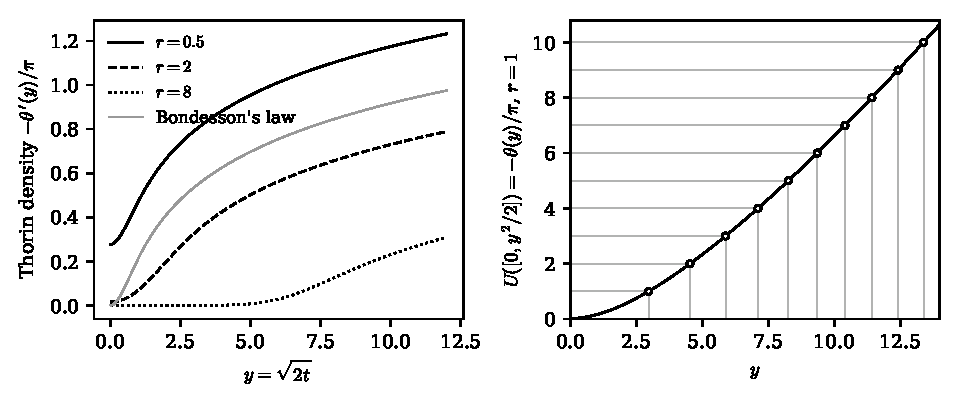
\includegraphics[width=\textwidth]{figures/hw_thorin.pdf}
\caption[The Thorin measure of the Hartman Watson law]{Left: the Thorin density of the Hartman Watson law in the variable $y=\sqrt{2q}$, for three values of $r$, with that of Bondesson's law $e^{-\gamma_{\mathrm E}\nu}/\Gamma(1+\nu)$. Right: the Thorin distribution function at $r=1$; it takes the value $n$ exactly at the $n$th zero of P\'olya's function $K_{iy}(1)$, marked by circles.}
\label{fig:hwthorin}
\end{figure}

\begin{corollary}[the Wilson action is a Thorin mixture of heat kernels]\label{cor:wilsonthorin}
The mixing law $\tilde\Xi_\kappa$ in $e^{\kappa x}/Z(\kappa)=\int K_{2\xi}\,\tilde\Xi_\kappa(d\xi)$ is a generalized gamma convolution, with Thorin measure that of $\Xi_\kappa$ moved to the right by $\frac12$:
\[
\frac{I_n(\kappa)}{I_1(\kappa)}=\exp\Big(\frac1\pi\int_0^\infty\log\Big(1+\frac{n^2-1}{1+y^2}\Big)\phi_\kappa'(y)\,dy\Big).
\]
Its Thorin measure is supported on $[\frac12,\infty)$, so $\tilde\Xi_\kappa$ has exponential moments of every order below $\frac12$.
\end{corollary}

\begin{proof}
An exponential tilt $e^{-c\xi}$ of a generalized gamma convolution replaces $\log(1+s/q)$ by $\log\big(1+s/(q+c)\big)$. Here $c=\frac12$, $s=\frac12(n^2-1)$ and $q=\frac12y^2$.
\end{proof}

At $\kappa=2$ the right side, by the quadrature of \texttt{hw\_thorin.py}, gives $\log(I_2/I_1)=-0.8367$ and $\log(I_4/I_1)=-3.4457$ against the exact $-0.8367$ and $-3.4454$. The corollary answers the question the last section ended on. The gap $\frac34$ of a heat kernel at unit time, mixed over a law whose Thorin measure begins at $\frac12$, is how the Wilson law carries its own first character.

\paragraph{\normalfont\scshape The von Mises law and the extended class.} The theorem of Hartman and Watson was stated for spheres in every dimension, and on the circle it says that the von Mises law is a mixture of wrapped normal laws over $\Xi_\kappa$. A normal law with variance drawn from a generalized gamma convolution is an extended generalized gamma convolution in Thorin's and Bondesson's sense, so by Theorem~\ref{thm:hwggc} the von Mises law is such a law on the line, wrapped round the circle. On SU(2) the heat kernel takes the place of the normal law and the Wilson law that of the von Mises law. This is the sense in which Hartman's result of 1976 is a scale mixture of normals result of the extended kind: his complete monotonicity gives the mixture, and the theorem above places the mixing law in Thorin's class.

\paragraph{\normalfont\scshape Four links with the Riemann volumes.} The theorem sits closer to our \emph{Computing the Riemann Hypothesis} \cite{PS26a,PS26b,PS26c} than any other result of this book.

First, the substitution. The Polson $2\sin^2$ lemma, Lemma~\ref{lem:2sin2B}, passes from a transform in $w$ to a Thorin measure in $u=\frac12w^2$, and its kernel is $1-\cos(xy)=2\sin^2(\frac12xy)$ with $y=\sqrt{2z}$ in the notation of the lemma, where $x$ is the variable called $\omega$ below. Here $w$ is the order $\nu$ of the Bessel function and $u$ is $s$. If $\nu\mapsto I_\nu(r)$ has only real zeros $-a_k$, then
\[
-\log\frac{I_\nu(r)}{I_0(r)}=\frac{K_0(r)}{I_0(r)}\,\nu+\int_0^\infty\big(e^{-\nu\omega}+\nu\omega-1\big)\sum_ke^{-a_k\omega}\,\frac{d\omega}{\omega},
\]
a compensated transform of a positive measure, and the lemma gives the Thorin density at once as
\[
-\phi_r'(y)=\frac{K_0(r)}{I_0(r)}+\sum_k\frac{y^2}{a_k(a_k^2+y^2)} .
\]
Theorem~\ref{thm:hwggc} proves the positivity of the left side without knowing where the zeros are; the argument above shows only that none has real part above $-\frac12$. So it is an instance in which the conclusion of the lemma holds and the reality of the zeros behind it is, as far as we know, open, the reverse of the situation for the Riemann xi function, where one wants the zeros and has the lemma.

Second, the phase. In the Riemann volumes the Thorin measure of the reciprocal xi function at the centre is the counting measure of the zeros at $\frac12\gamma^2$, and its smooth part is the derivative of the phase of the gamma factor. Here the Thorin measure is exactly the derivative of a phase, $-\phi_r'(y)/\pi$, and for large $y$ that phase is $-\arg\Gamma(1+iy)+y\log\frac12r$: the same function, with density $\frac1\pi\log(2y/r)$ in place of $\frac1{2\pi}\log(T/2\pi)$.

Third, P\'olya. The imaginary part of $I_{iy}(r)$ is $-\sinh(\pi y)K_{iy}(r)/\pi$, and $K_{iy}(r)$ is the function whose zeros in $y$ P\'olya proved real in 1926, in his study of approximations to the xi function \cite{Po26}. Since the phase is strictly decreasing it passes through the multiples of $\pi$ once each, and exactly at those zeros. Hence
\[
\#\{0<y\le Y:\ K_{iy}(r)=0\}=\big\lfloor U_r\big([0,\tfrac12Y^2]\big)\big\rfloor :
\]
the Thorin distribution function of the Hartman Watson law counts P\'olya's zeros. At $r=1$ (\texttt{hw\_thorin.py}) the first ten zeros are at $y=2.9625$, $4.5345$, \dots, $13.3859$, and $-\phi_1/\pi$ there is $1.0000$, $2.0000$, \dots, $10.0000$. It is a Riemann and von Mangoldt formula for P\'olya's function with no error term, and it is the Hermite and Biehler picture of the volumes: $I_{iy}$ is the structure function and $K_{iy}$ its odd part.

Fourth, Bondesson's letter. As $r\to0$, $I_\nu(r)/I_0(r)$ tends to $(r/2)^\nu/\Gamma(1+\nu)$, which is $e^{-\gamma_{\mathrm E}\nu}/\Gamma(1+\nu)$ times $e^{-(\log(2/r)-\gamma_{\mathrm E})\nu}$. The first factor, in $\nu=\sqrt{2s}$, is up to scale the law of Bondesson's letter of 2016 printed in the first Riemann volume \cite{PS26a}, with Thorin density $\frac1\pi\big(\gamma_{\mathrm E}+\operatorname{Re}\psi(1+iy)\big)$; the second is the hitting time of a level by Brownian motion. So the Hartman Watson laws are a one parameter family that ends, at small $r$, in Bondesson's law convolved with a stable law of index one half, and at every $r$ the density at $y=0$ is $K_0(r)/\pi I_0(r)$, the stable part.

\paragraph{\normalfont\scshape What it gives the mass gap.} Not the gap. It relates the two actions of this book, which Section~\ref{ch:kingman} found to behave differently at the first rung, by a mixture inside Thorin's class: any statement proved for heat kernels that is linear in the law, or stable under such mixtures, passes to Wilson's action. Which of the statements of this book are of that kind is the question to ask next; the contraction of Theorem~\ref{thm:scaledmlr} is not, since bond moving is not linear.

\section{A sharper criterion: Schur and Szeg\H o}\label{sec:szego}\index{Schur Szeg\H o composition}\index{multiplier sequence}\index{de la Vall\'ee Poussin kernel}

Theorem~\ref{thm:zeros} asks that one factor have an antiderivative in $\mathcal L$, and most members of $\mathcal L$ have none: of random polynomials in $\mathcal L$ of degree $3$, $6$ and $12$, about $81$, $28$ and $3$ per cent do (\texttt{szego\_criterion.py}). The hypothesis can be weakened a great deal by using, in place of Malo's theorem, the composition theorem from which it descends.

\begin{theorem}[Schur and Szeg\H o \cite{Sz22}]\label{thm:schurszego}
If $A(z)=\sum_{k=0}^n\binom nka_kz^k$ has only real zeros and $B(z)=\sum_{k=0}^n\binom nkb_kz^k$ has only real zeros, all of the same sign, then $\sum_{k=0}^n\binom nka_kb_kz^k$ has only real zeros.
\end{theorem}

In the language of P\'olya and Schur, $B$ is the Jensen polynomial of the sequence $(b_k)$, and the theorem says that a sequence whose Jensen polynomial of degree $n$ has real zeros of one sign multiplies the coefficients of every real polynomial of degree $n$ with real zeros into another such. Malo's theorem is the case in which $\sum b_kz^k$ itself has real zeros of one sign.

\begin{theorem}[the smoothed criterion]\label{thm:szegocriterion}
Let $f,g\in\mathcal L$ be polynomials of degrees $d$ and $D$. If $f*f_D\in\mathcal L'$, or if $g*f_d\in\mathcal L'$, then $f*g\in\mathcal L$.
\end{theorem}

\begin{proof}
Suppose $f*f_D\in\mathcal L'$, and put $N=D+1$. As in the proof of Theorem~\ref{thm:zeros}, $P(z)=z^N\tilde g(z)$ is a polynomial of degree $2N$ with only real zeros, and by Lemma~\ref{lem:circle} the coefficients of $z^N\,\widetilde{f*g}$ are those of $P$ multiplied by $q_m=a_{|m|}/|m|$ at the power $z^{N+m}$, $m\ne0$, where $f=\sum a_n\chi_n$; the coefficient of $z^N$ in $P$ is zero, so $q_0$ is at our disposal. The Jensen polynomial of this sequence is
\[
\sum_{m=-N}^{N}\binom{2N}{N+m}q_m\,z^{N+m}=z^N\Big(c+2\sum_{m\ge1}\binom{2N}{N+m}\frac{a_m}{m}\,T_m(x)\Big),
\]
with $x=\frac12(z+z^{-1})$. Since $(1+x)^N=2^{-N}\sum_m\binom{2N}{N+m}z^m$, the density $f_D\propto(1+x)^{N-1}$ has character coefficients proportional to $m\binom{2N}{N+m}$, so $f*f_D$ is proportional to $\sum_m\binom{2N}{N+m}a_m\chi_m$, and the bracket is an antiderivative in $x$ of a multiple of $f*f_D$, with $c$ free. By hypothesis $c$ can be chosen so that the bracket is in $\mathcal L$; then the Jensen polynomial has only negative zeros and a possible zero at the origin, and Theorem~\ref{thm:schurszego} gives $z^N\,\widetilde{f*g}$ only real zeros. So the zeros of $f*g$ in $x$ are real and outside $(-1,1)$, and since $f*g\in\mathcal M$ they are at most $-1$. The other case is the same with $f$ and $g$ exchanged.
\end{proof}

Three remarks on what has been gained.

\emph{It contains the old theorem.} If $f\in\mathcal L'$ then $f*f_D\in\mathcal L'$ by Theorem~\ref{thm:zeros}(ii), since every $f_D$ is in $\mathcal L'$.

\emph{It is a statement about one function.} The hypothesis does not involve $g$ beyond its degree. And it gives more than was asked: when it holds, convolution with $f$ carries every real polynomial of degree $2D+2$ in $z$ with real zeros to another, not only those that come from $\mathcal L$. The laws $f$ for which this is so, for a given $D$, are closed under convolution with each other, because their multiplier sequences multiply termwise.

\emph{It is a smoothing.} The binomial weights are the Fourier coefficients of $\cos^{2N}(\theta/2)$, the kernel of de la Vall\'ee Poussin, so the bracket is the antiderivative of $f$ smoothed on the circle by that kernel, which is close to a heat kernel at time $4/N$. An antiderivative of a function with real zeros need not have real zeros; the criterion asks only that it have them after a smoothing whose strength is matched to the degree of the other factor. This is de Bruijn's phenomenon again: smoothing moves zeros onto the real axis.

\begin{figure}[t]
\centering
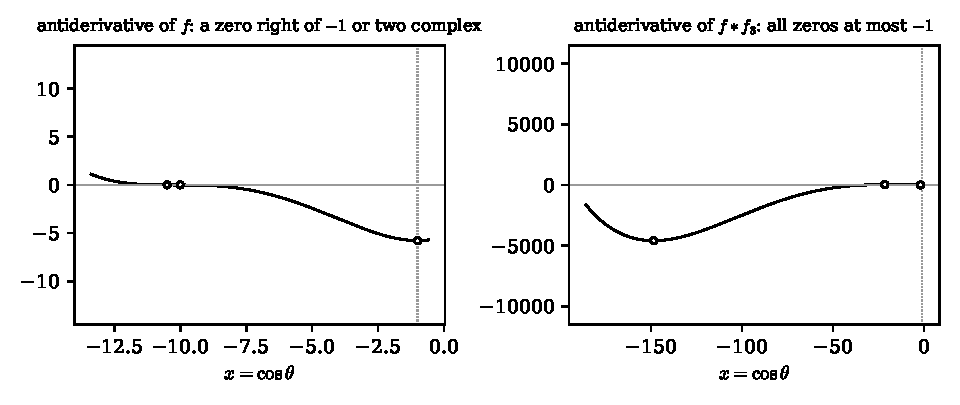
\includegraphics[width=\textwidth]{figures/szego_smoothing.pdf}
\caption[Smoothing makes the antiderivative real rooted]{The law $f=(1+x)(1+x/10)(1+x/10.5)$ is in $\mathcal L$ and not in $\mathcal L'$. Left: its antiderivative, with the constant chosen as well as it can be; the circles are the zeros of $f$, and the fourth zero falls to the right of $-1$. Right: the antiderivative of $f*f_3$, which has four real zeros at most $-1$, so that Theorem~\ref{thm:szegocriterion} applies to $f*g$ for every cubic $g\in\mathcal L$.}
\label{fig:szego}
\end{figure}

Does the hypothesis hold? In every case we have tried, when the degrees are comparable.

\begin{center}
\small
\begin{tabular}{cccc}
\toprule
degree of $f$ & $D$ & $f\in\mathcal L'$ & $f*f_D\in\mathcal L'$ \\ \midrule
$3$ & $3$ & $0.81$ & $1.00$ \\
$6$ & $6$ & $0.28$ & $1.00$ \\
$9$ & $9$ & $0.18$ & $1.00$ \\
$12$ & $12$ & $0.03$ & $1.00$ \\
$4$ & $12$ & $0.49$ & $1.00$ \\
\bottomrule
\end{tabular}
\end{center}

Each row (\texttt{szego\_criterion.py}, seed $3$) is $120$ polynomials in $\mathcal L$ with zeros spread over four decades, split into a cluster near $-1$ and a cluster far away, or of two zeros with high multiplicity, in $120$ digit arithmetic. In the other direction, for $g$ of degree $6$ to $12$ and $d$ from $1$ to $5$, $g*f_d$ was in $\mathcal L'$ in all $480$ trials, $80$ for each of six pairs $(\deg g,d)$. The laws that the old theorem could not reach are covered: for bond moved laws $\rho^k$ with $k=2$ and $4$, with two or more distinct zeros, all of even multiplicity, so that they are never in $\mathcal L'$, the smoothed law $\rho^k*f_d$ was in $\mathcal L'$ in each of six cases, among them $\rho=(1+x/1.2)(1+x/2)(1+x/5)$ and $\rho=(1+x/1.001)(1+x/1000)$. The hypothesis $f*f_D\in\mathcal L'$ does fail when $D$ is much larger than the degree of $f$, as it must, since $f*f_D\to f$: for $f=(1+x)(1+x/10)(1+x/10.5)$ it holds for $D=3$, $6$ and $12$ and fails for $D=24$. That is why the theorem has two cases, and the second, in which the factor of higher degree is smoothed by the lower, is the one that has not failed.

\begin{conjecture}[smoothing]\label{conj:smoothing}
If $g\in\mathcal L$ is a polynomial and $d\le\deg g$, then $g*f_d\in\mathcal L'$: the convolution of $g$ with $(1+\cos\theta)^d$ has an antiderivative in $\cos\theta$ with only real zeros, all at most $-1$.
\end{conjecture}

By Theorem~\ref{thm:szegocriterion}, Conjecture~\ref{conj:smoothing} implies Conjecture~\ref{conj:Lclosed} for polynomials, and for their limits by the estimate in the proof of Theorem~\ref{thm:zeros}(iii), applied to two factors, for which the products $a_nb_n/n$ of character coefficients are $O(R^{-2n})$ for every $R$. It is a statement about a single function and a single explicit kernel in place of a statement about all pairs, and for $d\le2$ its second half is automatic, since every polynomial of degree at most two in $\mathcal L$ is in $\mathcal L'$. We have not proved it. Two attempts that fail are worth a line each. Laguerre's theorem, that an entire function of the Laguerre and P\'olya class without zeros in $[0,n]$ gives a multiplier for polynomials of degree $n$, would do it if the character coefficients $b_m/m$ had such an interpolation in $m$; the natural even interpolation, a combination of the functions $1/\Gamma(J+1-s)\Gamma(J+1+s)$, has complex zeros in $214$ of $300$ random trials (\texttt{zeros\_checks.py}, seed $2$: $g$ of degree $2$ to $6$ with $\gamma-1=10^U$, $U$ uniform on $(-2,3)$, and the constant of integration fixed by $G(-1)=0$). And writing the convolution as a mixture over an auxiliary variable of polynomials each of which has real zeros, which can be done explicitly, proves nothing, since mixtures do not keep real zeros.

\section{The radial flow, and a criterion by signs}\label{sec:radial}\index{radial flow}\index{interlacing}

A third approach to Conjecture~\ref{conj:Lclosed} compares the convolution on SU(2) with the convolution on the circle, for which the conjecture is Malo's theorem. For class functions write
\[
(f\circledast g)(\cos\theta)=\frac1{2\pi}\int_0^{2\pi}f(\cos\psi)\,g(\cos(\theta-\psi))\,d\psi,
\]
and put $\mathcal D_sf(x)=f(sx)$ and $Ef=x\,f'(x)$.
If $f,g\in\mathcal L$ then $\mathcal D_sf,\mathcal D_sg\in\mathcal L$ for $0<s\le1$, their zeros being those of $f$ and $g$ divided by $s$; and $f\circledast g$ has only real zeros, all at most $-1$, because in the variable $z$ it is the Hadamard product of two polynomials with negative zeros.

\begin{theorem}[radial flow]\label{thm:radialflow}
For class functions $f,g$ and $0<s\le1$,
\[
s^2\,(\mathcal D_sf*\mathcal D_sg)=\int_0^s2\varrho\,(\mathcal D_\varrho f\circledast \mathcal D_\varrho g)\,d\varrho,\qquad\frac{d}{ds}\big[s^2(\mathcal D_sf*\mathcal D_sg)\big]=2s\,(\mathcal D_sf\circledast \mathcal D_sg),
\]
and
\[
f\circledast g=f*g+\tfrac12\,(Ef)*g+\tfrac12\,f*(Eg).
\]
If $f=\prod_{i\le d}(1+x/\gamma_i)$ and $g=\prod_{k\le D}(1+x/\delta_k)$, and $f_{\setminus i}$, $g_{\setminus k}$ denote the products with one factor removed, then
\[
\Big(1+\frac{d+D}{2}\Big)\,f*g=f\circledast g+\frac12\sum_{i=1}^df_{\setminus i}*g+\frac12\sum_{k=1}^Df*g_{\setminus k}.
\]
\end{theorem}

\begin{proof}
By Lemma~\ref{lem:ellipse} and its proof, $(f*g)(\cos\theta)=\frac1\pi\int_{|p|<1}f(p\cdot u)\,g(p\cdot e_\theta)\,d^2p$ over the unit disc, with $u$ and $e_\theta$ unit vectors at angle $\theta$. Replacing $f,g$ by $\mathcal D_sf,\mathcal D_sg$ and $p$ by $p/s$ gives $s^2(\mathcal D_sf*\mathcal D_sg)=\frac1\pi\int_{|p|<s}f(p\cdot u)g(p\cdot e_\theta)\,d^2p$, and in polar coordinates the integral over the circle of radius $\varrho$ is $2\pi\,(\mathcal D_\varrho f\circledast \mathcal D_\varrho g)$. That is the first identity. For the second apply the divergence theorem on the unit disc to the field $p\,f(p\cdot u)g(p\cdot e_\theta)$, whose divergence is $2fg+(Ef)g+f(Eg)$ and whose flux through the boundary is $2\pi(f\circledast g)$. For the third, $Ef=\sum_ixf/(x+\gamma_i)=d\,f-\sum_if_{\setminus i}$.
\end{proof}

So the convolution on SU(2) is the running average, over the radius, of convolutions on the circle of dilated laws, each of which has real zeros. A mixture of polynomials with real zeros need not have real zeros; but this mixture is a flow, and a flow keeps real zeros as long as the polynomial and its derivative along the flow interlace.

\begin{proposition}[the flat limit]\label{prop:flatlimit}
Let $f=\sum_kf_kx^k$ and $g=\sum_kg_kx^k$ be polynomials in $\mathcal L$. As $s\to0$ the zeros of $\mathcal D_sf*\mathcal D_sg$ are asymptotic to $y_i/s^2$, where the $y_i$ are the zeros of
\[
Q(y)=\sum_k\frac{f_kg_k}{k+1}\Big(\frac y2\Big)^k,
\]
and $Q$ has only real negative zeros. The zeros of $\mathcal D_sf\circledast \mathcal D_sg$ are asymptotic to those of $P(y)=\sum_kf_kg_k(y/2)^k$ divided by $s^2$, and $P=(yQ)'$, so the zeros of $P$ interlace those of $Q$.
\end{proposition}

\begin{proof}
The coefficient of $x^k$ in $E(u\cdot v)^j(e\cdot v)^{j'}$ over $S^3$ vanishes unless $j,j'\ge k$, and for $j=j'=k$ it is the number $k!$ of perfect matchings between the two groups times the constant $1/2^k(k+1)!$ of the proof of Theorem~\ref{thm:matching}; on the circle the constant is $1/2^kk!$. The lowest order in $s$ of the coefficient of $x^k$ is therefore $s^{2k}f_kg_k/2^k(k+1)$, and $s^{2k}f_kg_k/2^k$ on the circle. By Schur's theorem $\sum_kk!\,f_kg_ky^k$ has only real negative zeros, $f$ and $g$ having negative zeros, and $1/(k+1)!$ is a multiplier sequence of the first kind, by Laguerre's theorem. The last statement is Rolle's.
\end{proof}

\begin{theorem}[closure follows from the absence of a common zero]\label{thm:flowclosure}
Let $f,g\in\mathcal L$ be polynomials, and suppose the polynomial $Q$ of Proposition~\ref{prop:flatlimit} has simple zeros. If for no $s\in(0,1]$ do $\mathcal D_sf*\mathcal D_sg$ and $\mathcal D_sf\circledast \mathcal D_sg$ have a common zero, then $f*g\in\mathcal L$, and the zeros of $f\circledast g$ strictly interlace those of $f*g$, each zero of $f*g$ lying to the left of the corresponding zero of $f\circledast g$. In that case the zeros of $\mathcal D_sf*\mathcal D_sg$ increase strictly with $s$.
\end{theorem}

\begin{proof}
Put $\Phi_s=s^2(\mathcal D_sf*\mathcal D_sg)$ and $\Psi_s=\mathcal D_sf\circledast \mathcal D_sg$, polynomials in $x$ of the same degree with positive leading coefficients, and $\partial_s\Phi_s=2s\Psi_s$. By Proposition~\ref{prop:flatlimit}, for small $s$ the zeros of $\Phi_s$ are real and simple and strictly interlaced by those of $\Psi_s$. Let $s^*$ be the supremum of the $s$ up to which this holds. At $s^*$ the zeros of $\Phi$ are real and weakly interlaced by those of $\Psi$, which are real by Malo's theorem. A double zero of $\Phi_{s^*}$, or a failure of strictness, would put a zero of $\Psi_{s^*}$ on a zero of $\Phi_{s^*}$, which is excluded. So the interlacing is strict at $s^*$, and being an open condition it persists, whence $s^*=1$. With strict interlacing, $\Psi_s$ has at each zero of $\Phi_s$ the sign opposite to that of $\Phi_s'$, so every zero moves to the right.
\end{proof}

A second criterion uses the last identity of Theorem~\ref{thm:radialflow} and nothing else.

\begin{theorem}[a criterion by signs]\label{thm:signcriterion}
Let $f,g\in\mathcal L$ be polynomials of degrees $d$ and $D$, let $n=\min(d,D)$, and let $\psi_1>\psi_2>\dots>\psi_n$ be the zeros of $f\circledast g$, assumed simple. If each of the $d+D$ lower convolutions $f_{\setminus i}*g$ and $f*g_{\setminus k}$ has the sign $(-1)^{j-1}$ at $\psi_j$, for $j=1,\dots,n$, then $f*g$ has $n$ real zeros, one in each interval $(\psi_{j+1},\psi_j)$ and one to the left of $\psi_n$; in particular $f*g\in\mathcal L$.
\end{theorem}

\begin{proof}
At $\psi_j$ the right side of the identity is half the sum of the lower convolutions, so $f*g$ has the sign $(-1)^{j-1}$ there. It has degree $n$ and a positive leading coefficient, so its sign at $-\infty$ is $(-1)^n$, opposite to its sign at $\psi_n$. That gives $n$ changes of sign, and all the zeros are below $\psi_1\le-1$.
\end{proof}

The hypothesis says that each lower convolution, in which one factor has been removed from $f$ or from $g$, is interlaced by the circle convolution of the full pair. It is the natural statement to carry in an induction on $d+D$: the lower convolutions are in $\mathcal L$ by the inductive hypothesis, each is interlaced by its own circle convolution $f_{\setminus i}\circledast g$, and that in turn interlaces $f\circledast g$ because a Hadamard product with a polynomial with negative zeros preserves interlacing. What the induction lacks is the passage from these two interlacings to the third, of $f_{\setminus i}*g$ with $f\circledast g$: both have their $j$th zeros in the same gap of the zeros of $f_{\setminus i}\circledast g$, and the order of the two within the gap is what must be shown.

Both hypotheses hold in every case we have computed (\texttt{radial\_flow.py}), in $80$ digit arithmetic. Along the flow, for $60$ pairs of degrees $2$ to $8$ with zeros spread over five decades or repeated, at $40$ values of $s$ each, the zeros of $\mathcal D_sf*\mathcal D_sg$ were real, strictly interlaced by those of $\mathcal D_sf\circledast \mathcal D_sg$, and increasing in $s$; the smallest gap between a zero of one and the nearest zero of the other, relative to its size, was $0.064$, so a common zero was never approached. And the sign condition held for all $1037$ lower convolutions of $120$ pairs. The identities of Theorem~\ref{thm:radialflow} hold to the precision of the arithmetic, and at $s=\frac1{200}$ the scaled zeros agree with those of $Q$ to five figures.

\begin{conjecture}[interlacing]\label{conj:interlacing}
For polynomials $f,g\in\mathcal L$ the zeros of the circle convolution $f\circledast g$ strictly interlace those of the SU(2) convolution $f*g$, each zero of $f*g$ lying to the left of the corresponding zero of $f\circledast g$.
\end{conjecture}

Applied to all dilations of a pair, Conjecture~\ref{conj:interlacing} excludes a common zero, so by Theorem~\ref{thm:flowclosure}, a perturbation that makes $Q$ simple, and the same limit estimate it implies Conjecture~\ref{conj:Lclosed}; and it is implied by the sign condition of Theorem~\ref{thm:signcriterion}. The conjecture of closure has thus been reduced three times, to a smoothing statement about one law, to the reality of zeros of a matching polynomial in a partial variable (Chapter~\ref{ch:theta}), and now to a statement with no reality in it at all: that two explicit polynomials, both of which may be assumed to have real zeros at every earlier stage of a flow, never vanish together.

\section{What is conjectured}

The exact ladder needs more. Bond moving raises $\rho$ to a power, which keeps it in $\mathcal L$ and multiplies the multiplicity of each zero by $k$. But a function with two or more distinct zeros, all of even multiplicity, is the derivative of a monotone function, which has one real zero and is not in $\mathcal L$; so bond moved laws with even $k$ are in $\mathcal L$ and not in $\mathcal L'$, and Theorem~\ref{thm:zeros} does not apply to their convolution with themselves. Theorem~\ref{thm:szegocriterion} does apply whenever its hypothesis can be checked, and it has held in every case tried; what is missing is a proof that it always holds.

\begin{conjecture}\label{conj:Lclosed}
The class $\mathcal L$ is closed under convolution on SU(2). Hence it is preserved by the exact Migdal Kadanoff ladder: at every rung, from a heat kernel or a Wilson law, the density of a link is a product $\prod_m(1+\cos\theta/\gamma_m)$ with $\gamma_m\ge1$.
\end{conjecture}

The evidence, from \texttt{real\_zeros.py} and \texttt{zeros\_adversarial.py}:
\begin{itemize}
\item Three hundred random pairs of polynomials in $\mathcal L$ of degrees up to twelve, with zeros clustered near $-1$, spread, or far away, neither required to be in $\mathcal L'$: every convolution is in $\mathcal L$. The largest zero found was $-1.040$.
\item An adversarial search aimed at the case the theorem does not cover, both factors with repeated zeros allowed: $260$ pairs of the form $\prod_i(1+x/\gamma_i)^{m_i}$ with multiplicities from one to four and zeros clustered within $10^{-3}$ of $-1$, spread, or as far as $-10^4$, in $160$ digit arithmetic. No convolution leaves the class.
\item Exact rungs of the ladder in polynomial arithmetic, power four followed by a fourfold convolution. From $f_3$: degree $12$ with largest zero $-1.190$, then degree $48$ with largest zero $-1.311$, all zeros real. From $(1+x/1.2)(1+x/2)(1+x/5)$: largest zeros $-1.588$ and $-2.324$, all zeros real. The second rungs need four hundred digits, since the leading coefficient is below $10^{-400}$ times the constant term.
\item The first rung from a heat kernel, with the product formula cut to its first five or six factors: all zeros real, the largest at $-2.657$ for $t=2$, where the heat kernel's was $-1.679$, and at $-1.224$ for $t=1$, where it was $-1.142$.
\item With $k=2$, the three dimensional case, from $(1+x/1.05)(1+x/9)$: the largest zero is $-8.48$ after one rung, $-1.8\times10^4$ after two and $-4.0\times10^{17}$ after three.
\end{itemize}

The last item shows what the conjecture would give. If the ladder acts on $\mathcal L$, it is a dynamical system on the zeros: bond moving multiplies their multiplicities and decimation moves them. A law is close to Haar measure when its zeros are far to the left, and close to the unit mass when they crowd toward $-1$. Confinement is the escape of the zeros to infinity, and in the three dimensional ladder of the last item, from one starting law and over three rungs, one sees it happen at a doubly exponential rate.

\paragraph{\normalfont\scshape The largest zero as a coupling.} By Theorem~\ref{thm:product} the largest zero $-\gamma_1(t)$ of the heat kernel moves monotonically to the left as $t$ grows, so $\gamma_1$ is a coupling in its own right, and one that is defined for every member of $\mathcal L$ whether or not it is a heat kernel; $1/\gamma_1$ is the largest Bernoulli parameter of the count. In the heat kernel computations above a rung of the exact ladder moves the largest zero to the left. A Wilson law has all its zeros at infinity, and a rung brings them in to finite distance, which is the gain of order recorded in Table~\ref{tab:notmonotone}. Whether $\gamma_1$ increases at every rung once the zeros are finite is a sharper form of the contraction question than any we have had, and we leave it open.

\paragraph{\normalfont\scshape Why the standard machinery does not close the gap.} We tried to prove the conjecture and did not succeed, and the way the attempt fails is worth recording. The modern route to theorems of this kind is the characterisation by Borcea and Br\"and\'en~\cite{BB09a,BB09b} of linear operators that preserve real zeros, through the stability of a symbol in two variables, together with the coincidence theorem of Grace, Walsh~\cite{Wa22} and Szeg\H o. Here the operator is $f\mapsto f*g$ and the symbol is $(\zeta,x)\mapsto\big((\zeta+x)^n*g\big)(x)$. Already for $g=1+x$ and $n=2$ the symbol is $\zeta^2+\frac12\zeta x+\frac14$, whose two roots in $\zeta$ lie on opposite sides of the real axis when $x$ is not real; in $720$ random trials (\texttt{zeros\_checks.py}, seed $1$), with $g$ a product of one to six factors $1+x/\gamma$, $\gamma-1=10^U$ for $U$ uniform on $(-2,3)$, $n$ from $2$ to $6$, and $x$ with real part uniform on $(-3,3)$ and imaginary part uniform on $(0.1,3)$, the symbol had a root in the closed upper half plane in $667$. The operator does not preserve real zeros in general: $x^2$ has real zeros and $x^2*(1+x)^2=\frac{x^2}{12}+\frac7{24}$ has none. It preserves, if the conjecture is right, only the smaller class of zeros at most $-1$, and a proof must use that the zeros of both factors lie beyond the edge of the group, where $\cos\theta=-\cosh\eta$ and the characters are hyperbolic. This is the content of Open problem~\ref{op:malo}.

The conjecture would also settle Open problem~\ref{op:logconcave} for laws in $\mathcal L$: sums of independent Bernoulli variables are log concave, so the count would be log concave at every rung, and more.

\begin{problem}\label{op:malo}
Prove Conjecture~\ref{conj:smoothing} or Conjecture~\ref{conj:interlacing}, or directly a theorem of Malo type for the pairing of Lemma~\ref{lem:circle} when neither factor has an antiderivative in $\mathcal L$: if $f$ and $g$ have only negative zeros in $z$, then $\sum_{n\ne0}\operatorname{sgn}(n)\,a_{|n|}b_{|n|}z^n/|n|$ vanishes only at $\pm1$ and on the negative axis.
\end{problem}

\section{Where this sits}

The book began with a positivity question, whether certain reciprocals are Laplace transforms of positive measures, and with the observation that such questions are questions about the location of zeros. It has come back to that. Chapter~\ref{ch:kacyang} looks for zero free sectors of partition functions in the coupling. This chapter finds real zeros of the link density in the angle. The two are different variables, and the second is the more tractable: the zeros in $\cos\theta$ are real for the heat kernel by the triple product, stay real under heat flow by Malo's theorem, and appear to stay real under the whole ladder.

It should be said again that none of this touches $\mathbb Z^4$. But a Lee Yang property has a feature that the likelihood ratio order lacks: it is a property of one function, not a comparison of two, and it passes to products over plaquettes without change. The Wilson measure on any lattice is a product over plaquettes of members of the closure of $\mathcal L$. Whether integration over links preserves a multivariate form of the property, as integration over spins does in the Lee Yang theorem \cite{LY52} and in the Asano contraction \cite{As70}, is the form of the comparison problem that this chapter suggests.

\section*{Exercises}
\begin{enumerate}
\item Verify Lemma~\ref{lem:circle} for $f=g=1+x$ and recover $f*g=1+x/4$ up to normalisation, a single zero at $-4$.
\item (Section~\ref{sec:twoclasses}.) Show that the antiderivative of $(1+x/\gamma_1)(1+x/\gamma_2)$ can be chosen in $\mathcal L$ for every $1\le\gamma_1\le\gamma_2$, and give three factors for which it cannot.
\item (Section~\ref{sec:twoclasses}.) Prove that the largest zero $-\gamma_1$ of $\rho\in\mathcal L$ satisfies $1/\gamma_1\le\E M_0\le d/\gamma_1$ when $\rho$ has degree $d$.
\item (Corollary~\ref{cor:coalzeros}.) For $f_a*f_b$, show that the sum of $1/\gamma_i(a,b)$ equals the mean of the count $M_0$, and compute it for $a=b=2$.
\item (Section~\ref{sec:circlecv}.) State the analogue of Theorem~\ref{thm:zeros} for the circle and prove it directly from Malo's theorem.
\end{enumerate}
